\section{Structure du projet :}

\subsection{Structure graphique Android et navigation :}
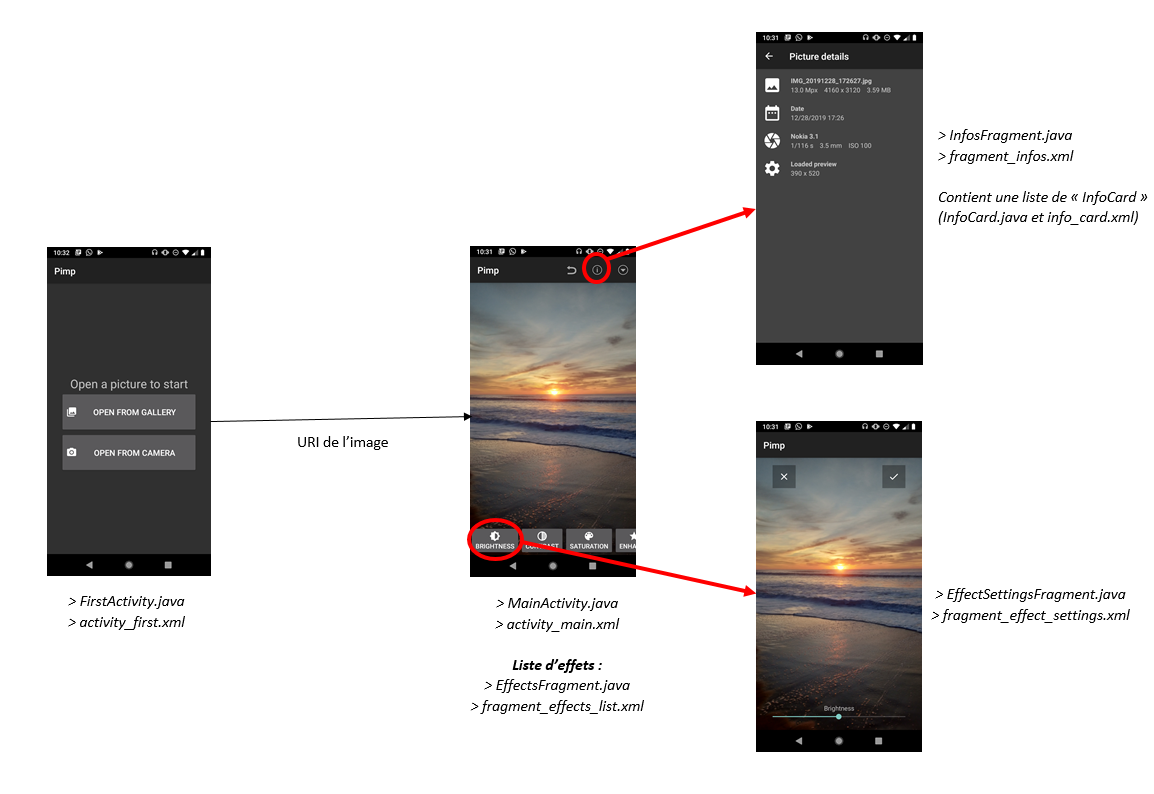
\includegraphics[width=1\textwidth]{report_src/app_flowchart_fragments.PNG}

Pour afficher certains éléments d'interface comme par exemple les informations de l'image (bouton \faInfoCircle) nous utilisons des \textbf{Fragment}. En effet une activité supplémentaire n'est pas nécessaire car cette petite partie de l'application ne correspond pas à un point d'entrée de l'application. Par ailleurs changer de fragment (plutôt que de changer directement de layout) pourrait faciliter l'implémentation d'une interface différente, pour tablette par exemple.
De même, la liste d'effets et leurs paramètres respectifs sont aussi contenus dans des fragments séparés. Cela permet de gérer plus simplement leur affichage et de clarifier le code.
\\

On notera que dans la structure actuelle de l'application, l'image actuellement éditée est contenue et manipulée depuis l'activité principale. Les fragments n'apportent à l'application que des éléments d'interface.
\\

Une seconde activité est cependant utilisée pour la page d'accueil à l'ouverture de l'application, cette \textbf{FirstActivity} utilise des méthodes génériques de \textbf{ActivityIO} afin de gérer l'ouverture de la galerie ou de la caméra. L'application reste dans cette activité tant qu'une \textbf{Uri} valable ($\approx$ chemin) n'a pas été sélectionnée. Ensuite cette Uri est transférée à \textbf{MainActivity} qui va alors charger cette première Image, en cas de problème de chargement l'application peut retourner dans FirstActivity.

\subsection{Classe \textbf{Image} :} \label{classeImage}
Cette classe a été conçu comme une alternative à l'utilisation directe de la classe \textbf{Bitmap} fournie par Android.
\\
Le coeur de la classe est évidement une instance de Bitmap, qu'il est possible de récupérer à tout moment. Par ailleurs la classe offre des fonctionnalités supplémentaires, parmi celle ci notamment la possibilité de restaurer l'image à son état au moment de sa création ou de son chargement via la méthode \textbf{reset()}, ou d'annuler les dernières modifications apportées par un effet grâce aux méthodes \textbf{quicksave()} et \textbf{discard()}.
\\

On notera la nécessité pour Image d'avoir la référence d'une Activité de l'application, en effet elle est requise à plusieurs moments par les librairies Android pour charger la Bitmap en mémoire.

\subsubsection{Classe \textbf{ImageInfo} :}
La classe Image \ref{classeImage} génère et garde une instance de la classe \textbf{ImageInfo}, cette classe contient un grand nombre de valeurs à propos de l'Image (dimensions, coordonnées GPS, date de prise de vue, ...).
\\
L'idée de cette classe était d'empaqueter toutes ces informations afin de faciliter le passage de ces informations à travers des Fragments ou des Activités (voir \ref{navig}). On notera que tous les accesseurs appliquent des opérations de formatage sur ces données, certaines opérations pourraient être déplacées dans les constructeurs si elles venaient à être utilisées régulièrement.

\subsection{Package \textbf{util} :}
Ce package contient de nombreuses classes contenant des méthodes statiques permettant une meilleur factorisation du code.
\\
La classe \textbf{Utils} offre par exemple des méthodes pour récupérer la taille de l'écran ou pour calculer un ratio de redimensionnement.
\\
La classe \textbf{BitmapIO} permet d'effectuer le chargement d'une Bitmap de plusieurs manières, depuis les resources ou un autre emplacement du téléphone, et avec la taille voulue.
\\
La classe \textbf{Effects} est une énumération des effets disponibles. Les enums sont passés en argument du chargement du fragment EffectSettings, afin d'afficher les bon paramètres d'effets.
\\
La classe \textbf{Kernels} contient tous les kernels de convolution (voir \ref{kernels}).